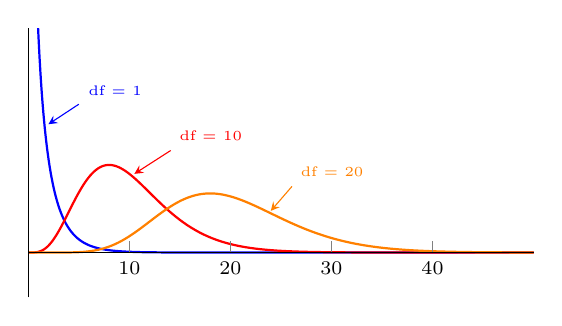
\begin{tikzpicture}[
    declare function={
        gamma(\z)=2.506628274631*sqrt(1/\z)+ 0.20888568*(1/\z)^(1.5)+ 0.00870357*(1/\z)^(2.5)- (174.2106599*(1/\z)^(3.5))/25920- (715.6423511*(1/\z)^(4.5))/1244160)*exp((-ln(1/\z)-1)*\z;
    },
    declare function={
        chisq(\x,\k) = ( ( (\x^(\k/2 - 1)) * exp(-\x/2) ) / ( (2^(\k/2))*gamma(\k/2) ) );
    }
  ]
    \begin{axis}[
        axis lines*=middle,
        no markers,
        domain=0.01:50,
        samples=500,
        xmin = 0, xmax = 50,
        ymin = -0.05, ymax = 0.25,
        xtick={0,10,...,40},
        ticklabel style={font=\scriptsize},
        ytick=\empty,
        grid = none,
        axis on top,
        height=5cm,
        width=8cm
      ]
      \addplot+[thick,blue] { chisq(x,1) };
      \addplot+[thick,red] { chisq(x,10) };
      \addplot+[thick,orange] { chisq(x,20) };
      \node[blue,right] (A) at (axis cs: 5,0.18) {\tiny df = 1};
      \node[red,right] (B) at (14,0.13) {\tiny df = 10};
      \node[orange,right] (C) at (26,0.09) {\tiny df = 20};
      \draw[blue,-stealth] (A.200) -- (axis cs: 2, {chisq(1.6,1)});
      \draw[red,-stealth] (B.200) -- (axis cs: 10.5, {chisq(10,10)});
      \draw[orange,-stealth] (C.200) -- (axis cs: 24, {chisq(23.5,20)});
    \end{axis}
\end{tikzpicture}